\section{Class Diagrams}

The system design is expected to adhere to the Layered and Repository
design patterns as outlined in \emph{\textbf{section 3.1}}.
Consequently, the system's classes are categorized into four distinct
groups.

\emph{View Classes} (Figure 21): These classes encompass the user
interface and user experience (UI/UX) components, along with methods for
handling user events. Each class inherits from a common class,
\emph{BaseLayout}, which encapsulates the components and methods shared
across all view classes.

\emph{Service Classes} (Figure 22): These classes contain methods for
processing the system's logic and business flow. Each class has a
specific responsibility and inherits from a class called
\emph{BaseService}, which encapsulates the methods and services common
to all service classes. The methods of service classes are made
available to view classes via an Application Programming Interface
(API).

\emph{DataLayer Classes} (Figure 23): Each class corresponds to a system
entity in the database. All DataLayer classes inherit from a class
called \emph{BaseDataLayer}, which provides all the methods needed to
interact with the database. It's important to note that a DataLayer
class can only interact with its corresponding entity in the database.

\emph{UnitOfWork} Class (Figure 23): This singular class contains
properties that are instances of DataLayer classes. The BaseService
class implements the UnitOfWork, enabling all service classes to access
the database. This class also includes methods to save changes or
rollback transactions in case of any exceptions at the end of an
application process.

This structure ensures a clear separation of concerns, promoting
maintainability and scalability in the system design.

\begin{figure}[H]
  \centering
  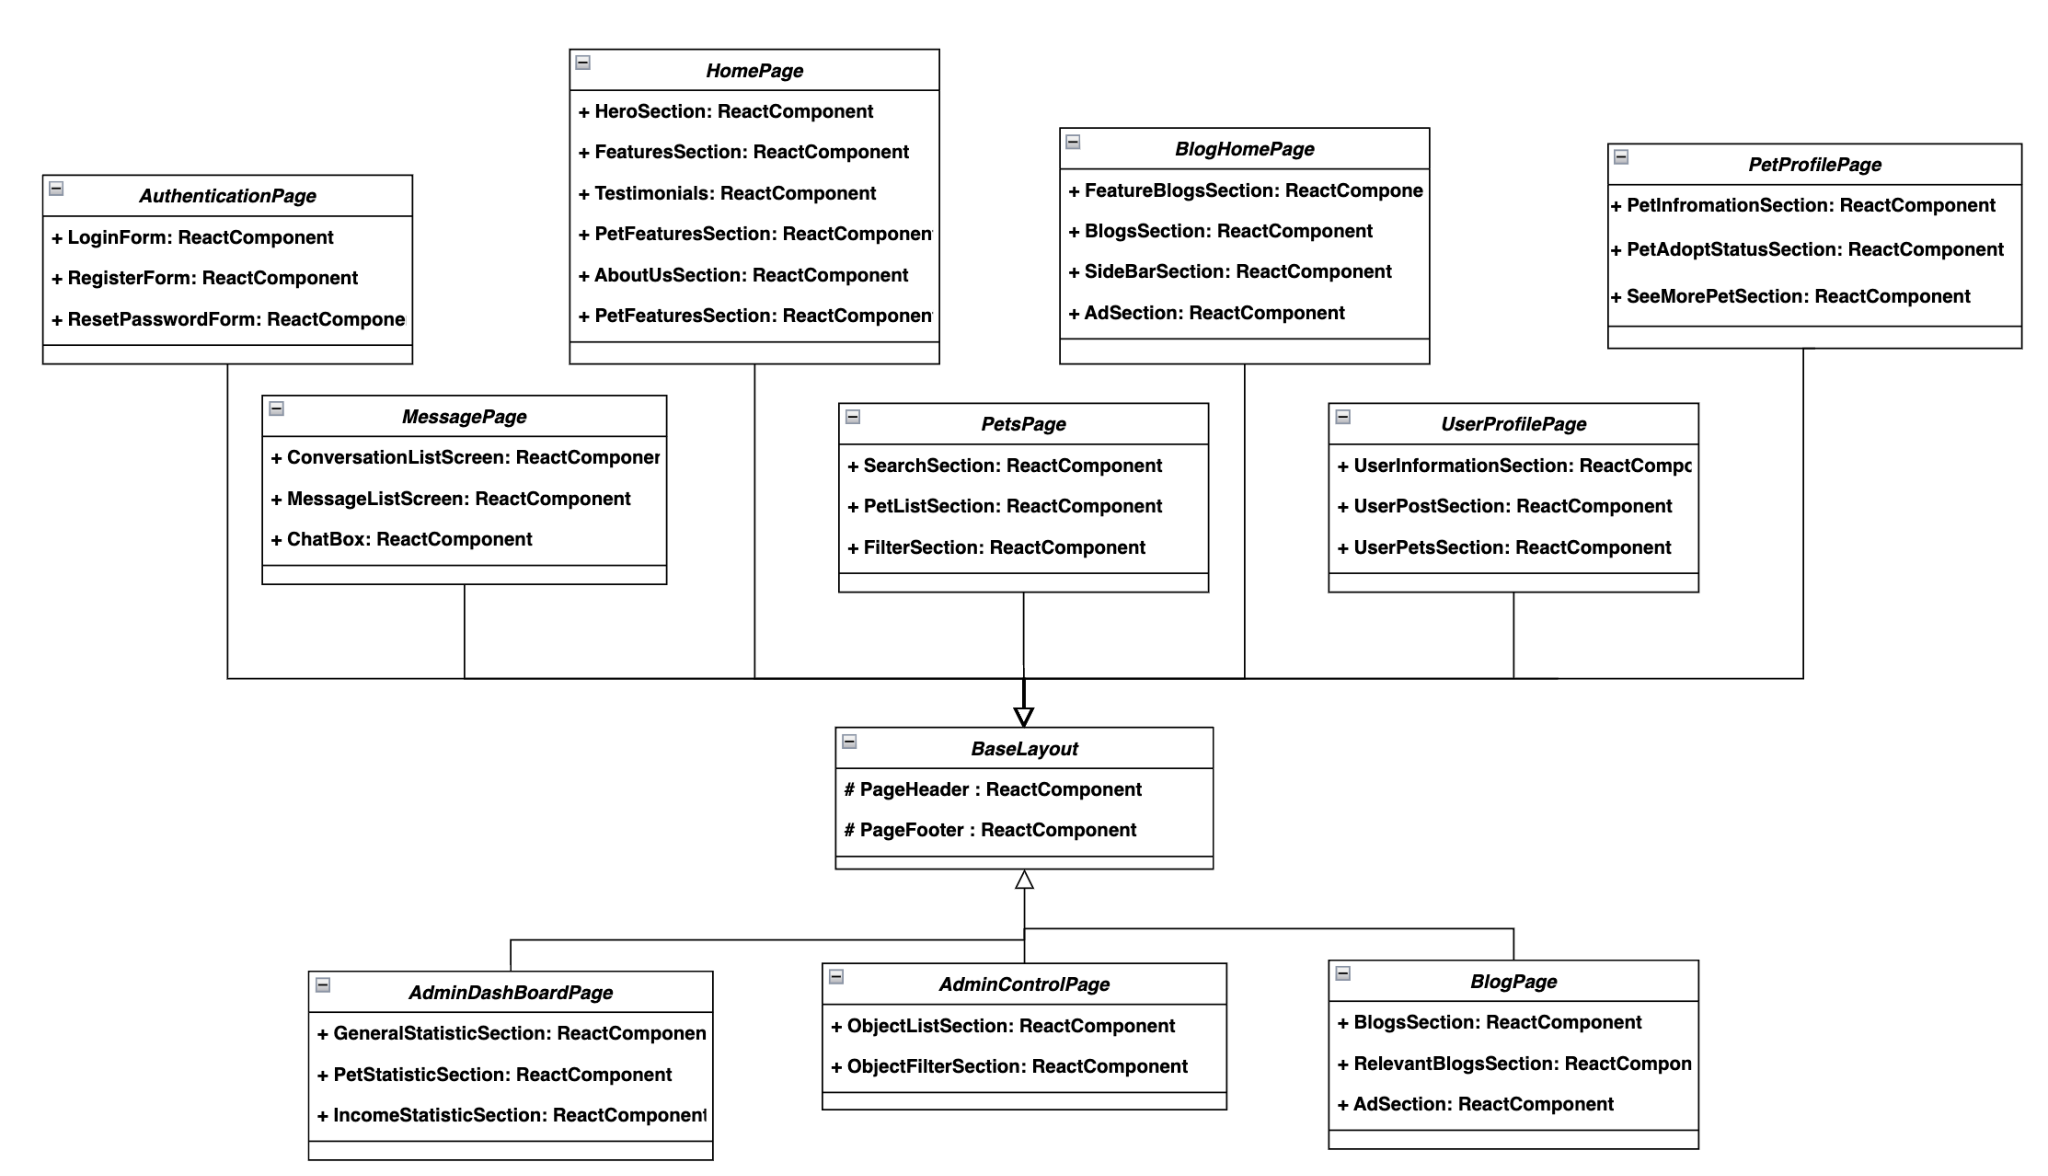
\includegraphics[angle=-90,width=0.8\textwidth]{Figures/view_class.png}
  \caption{View Classes}
  \label{fig:view-classes}
\end{figure}
\clearpage

\begin{figure}[H]
  \centering
  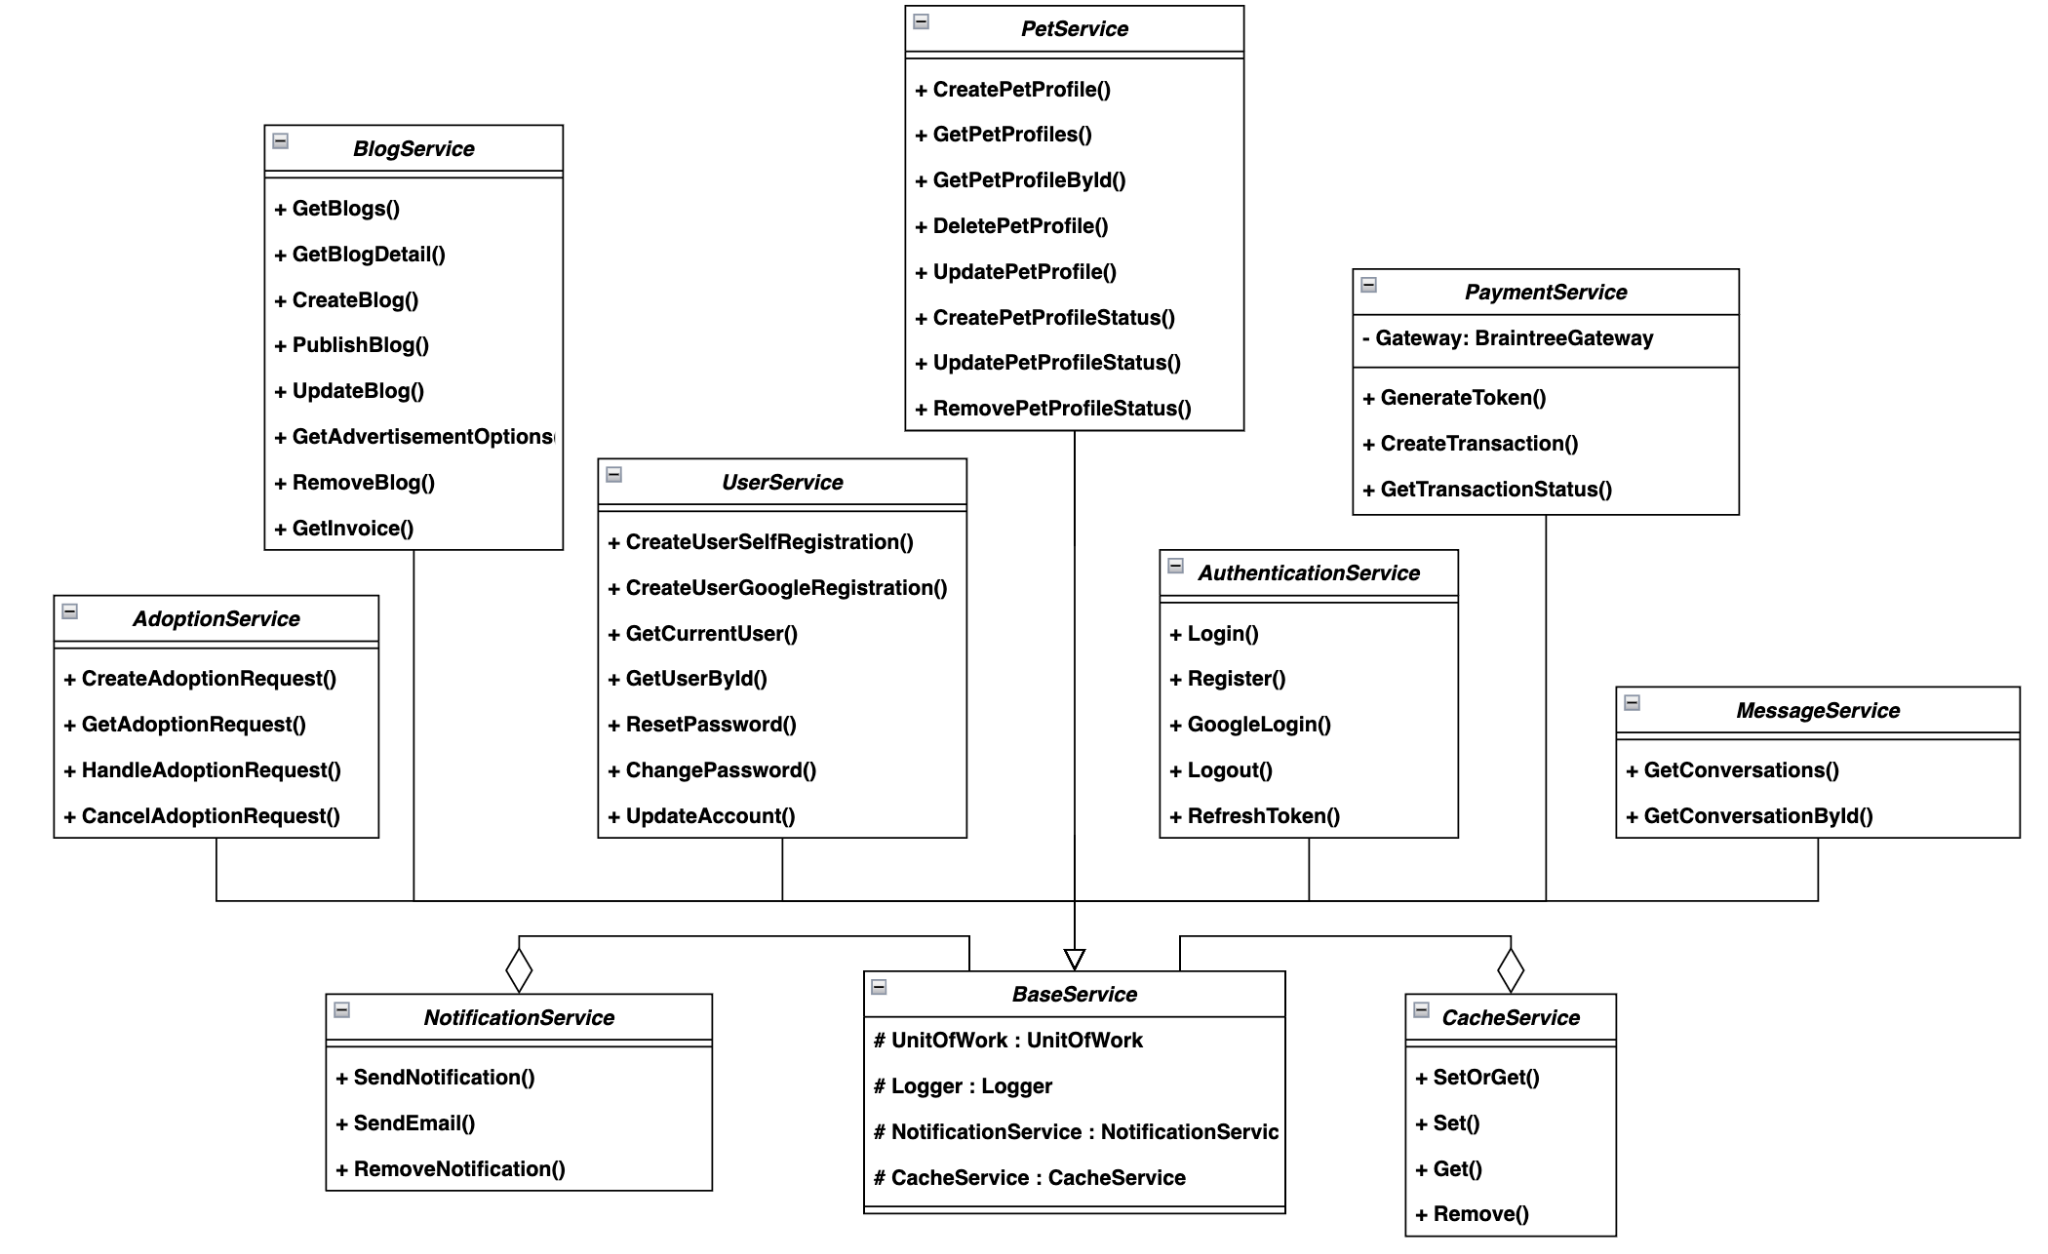
\includegraphics[angle=-90,width=0.8\textwidth]{Figures/service_class.png}
  \caption{Service Classes}
  \label{fig:service-classes}
\end{figure}

\begin{figure}[H]
  \centering
  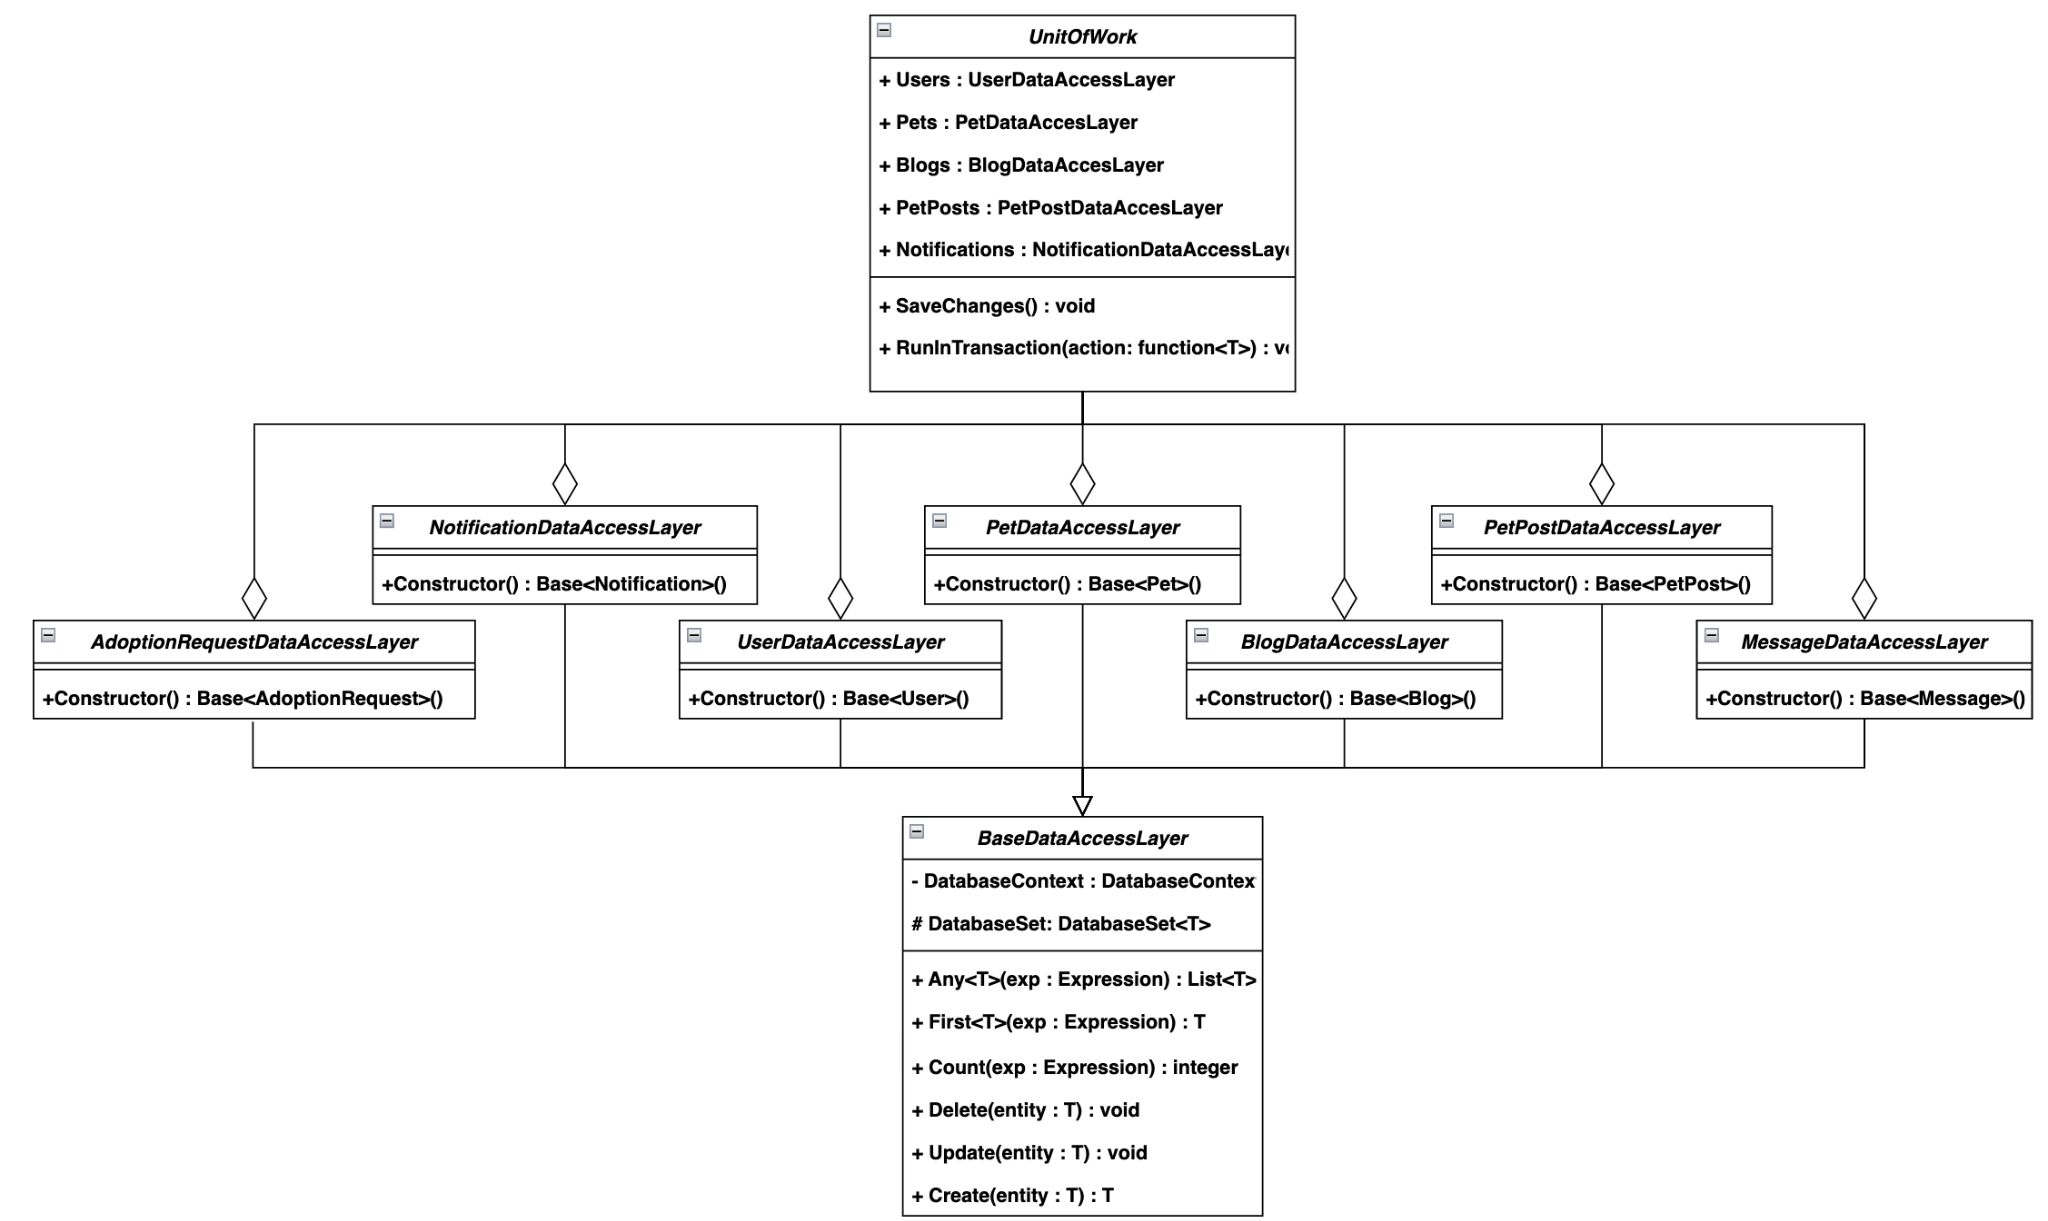
\includegraphics[angle=-90,width=0.8\textwidth]{Figures/uow_class.png}
  \caption{DataLayer Classes}
  \label{fig:datalayer-classes}
\end{figure}
\clearpage
